\documentclass{article}
\usepackage{ctex}
\usepackage{amsmath}
\usepackage{enumerate}
\usepackage{float}
\usepackage{tikz}
\bibliographystyle{unsrt}
\usepackage[top=2.5cm,bottom=2.5cm]{geometry}
\title{bresenham算法与边界填充算法在三维空间中的拓展}
\author{骆天奇}
\date{}


\begin{document}
	\maketitle
	\begin{abstract}
		本文根据经典的bresenham算法,讨论其在三维空间中对直线和椭圆的绘制算法;以及边界填充算法在三维空间中对封闭平面和封闭空间的填充算法。\\
		\textbf{关键字:} 计算机图形学, bresenham算法, 边界填充算法
	\end{abstract}
%	\newpage
%	\tableofcontents
	\section{Bresenham算法在三维空间中的应用与拓展}
\subsection{Bresenham算法简述\cite{计算机图形学基础}}
直线的绘制首先要考虑的是直线绘制的质量,有以下标准:
\begin{itemize}
    \item 直线要直,所选像素点应尽量靠近理想直线。
    \item 直线的端点要准确,保证绘制无定向性,即从$A$点到$B$点画一条直线同从$B$点到$A$点画一条直线应重合,且在绘制多条端点相连的直线时,不会因算法的累计错误造成断裂和不连接的情况。
    \item 相同设备下画线的速度应尽可能的快。
\end{itemize}
\subsubsection{中点Bresebham算法绘制二维直线\cite{计算机图形学基础}}
给定直线的两个端点$P_0(x_0,y_0)$和$P_1(x_1,y_1)$,可得到直线方程
\begin{align}
    F(x,y)=y-kx-b=0\\
    k=\frac{\Delta y}{\Delta x}=\frac{Y_1-Y_0}{X_1-X_0}
\end{align}
\par
这时直线将平面分为三个区域:对于直线上的点,$F(x,y)=0$;对于直线上方的点,$F(x,y)>0$;对于直线下方的点,$F(x,y)<0$,如图\ref{pic:直线将平面分为三个区域}所示。
\begin{figure}[H]
	\centering
	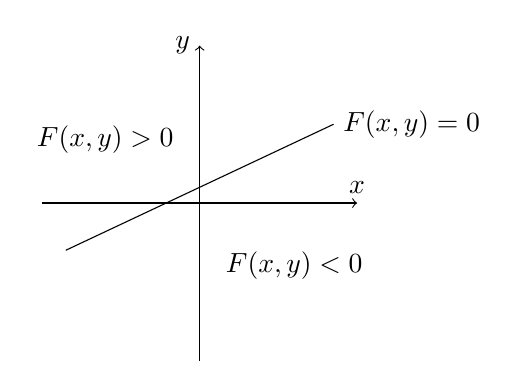
\begin{tikzpicture}[scale=1]
		\draw [->] (-2,0) -- (2,0) node[above]{$x$};
		\draw [->] (0,-2) -- (0,2) node[left]{$y$};
		\draw (-1.7,-.6) -- (1.7,1) node[right]{$F(x,y)=0$};
		\draw (-1.2,.5) node[above]{$F(x,y)>0$} (1.2,-.5) node[below]{$F(x,y)<0$};
	\end{tikzpicture}
	\caption{直线将平面分为三个区域}
	\label{pic:直线将平面分为三个区域}
\end{figure}
\par
由$Bresenham$提出的直线生成算法的基本原理是,每次在最大位移方向上走一步,而另一个方向是走步还是不走步取决于误差项的判别,如图\ref{pic:Brensemham算法生成直线的原理}所示。
\begin{figure}[H]
	\centering
	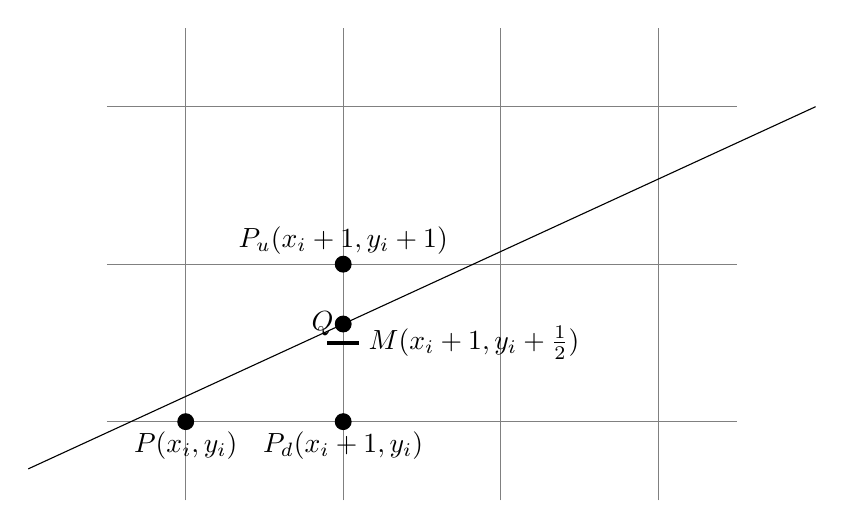
\begin{tikzpicture}[scale=2]
		\draw [help lines] (-.5,-.5) grid (3.5,2.5);
		\draw (-1,-.3) -- (4,2);
		\draw [fill]
		(0,0) circle [radius=0.05] node [below] {$P(x_i,y_i)$}
		(1,0) circle [radius=0.05] node [below] {$P_d(x_i+1,y_i)$}
		(1,1) circle [radius=0.05] node [above] {$P_u(x_i+1,y_i+1)$}
		(1,.5) node [right, xshift=.2cm] {$M(x_i+1,y_i+\frac{1}{2})$}
		(1,.62) circle [radius=0.05] node [left] {$Q$};
		\draw [ultra thick] (.9,.5) -- (1.1,.5);
	\end{tikzpicture}
	\caption{Brensemham算法生成直线的原理}
	\label{pic:Brensemham算法生成直线的原理}
\end{figure}
\par
假定$0\leq k \leq 1$,由于$x$是最大位移方向,因此每次在$x$方向上加$1$,$y$方向上或加$1$,或加$0$。
假设当前点是$P(x_i,y_i)$,则下一个点在$P_u(x_i+1,y_i+1)$与$P_u(x_i+1,y_i)$中选一。
以$M$表示$P_u$与$P_d$的中点,即$M(x_i+1,y_i+0.5)$。
又设$Q$是理想直线与垂直直线$x=x_i+1$的交点;
显然,若$M$在$Q$的下方,则$P_u(x_i+1,y_i+1)$离直线近,应取为下一个像素;
否则应取$P_d(x_i+1,y_i)$。
\par
如前所述,直线方程为$F(x,y)=y-kx-b$。欲判断$Q$在$M$的上方还是下方,只要把$M$代入$F(x,y)$,并判断它的符号即可。
\par
构造判式如下:
\begin{equation}
d_i=F(x_M,y_M)=F(x_i+1,y_i+0.5)=y_i+0.5-k(x_i+1)-b
\label{math:bresenham二维直线判别式}
\end{equation}
\par
当$d_i < 0$时,$M$在直线下方,故应取$P_u$。当$d_i \geq 0$时,则应取正右方的$P_d$,即
\[
y=\left\{
\begin{array}{ll}
y+1 & (d_i<0) \\
y & (d_i \geq 0)
\end{array}
\right.
\]
\par
现根据式(\ref{math:bresenham二维直线判别式})进行误差项的递推。如图\ref{pic:Bresenham算法误差项的递推}所示。
\begin{figure}
	\centering
	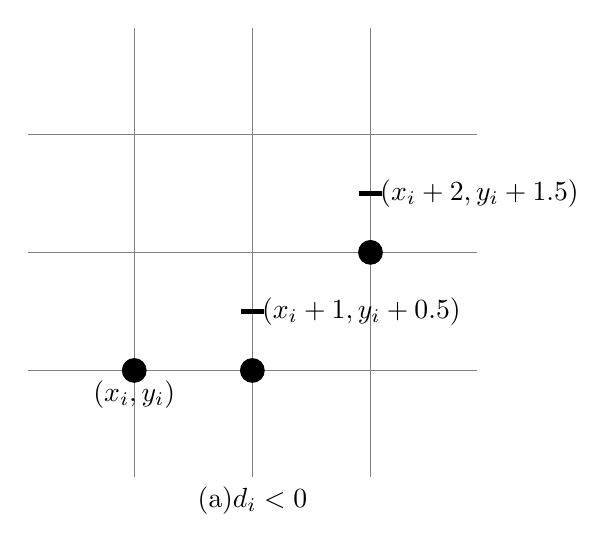
\begin{tikzpicture}[scale=1.5]
		\draw [help lines] (-.9,-.9) grid (2.9,2.9);
		\draw [fill]
		(0,0) circle [radius=0.1] node [below] {$(x_i,y_i)$}
		(1,.5) node [right] {$(x_i+1,y_i+0.5)$}
		(2,1.5) node [right] {$(x_i+2,y_i+1.5)$}
		(1,0) circle [radius=0.1]
		(2,1) circle [radius=0.1]
		(1,-.9) node [below] {(a)$d_i<0$};
		\draw [ultra thick]
		(.9,.5) -- (1.1,.5)
		(1.9,1.5) -- (2.1,1.5);
	\end{tikzpicture}
	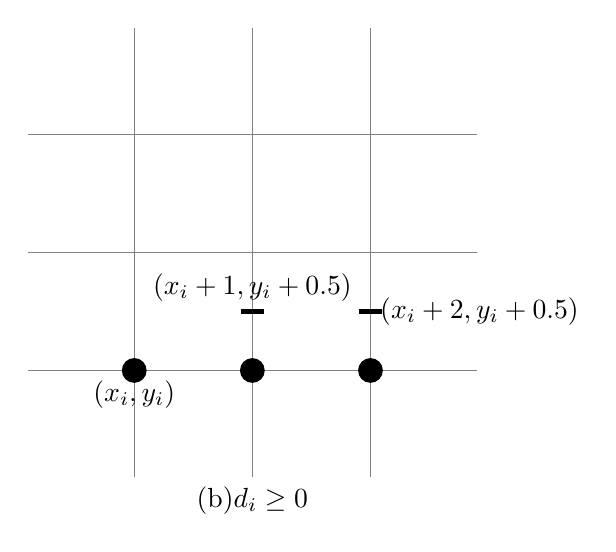
\begin{tikzpicture}[scale=1.5]
		\draw [help lines] (-.9,-.9) grid (2.9,2.9);
		\draw [fill]
		(0,0) circle [radius=0.1] node [below] {$(x_i,y_i)$}
		(1,.5) node [above] {$(x_i+1,y_i+0.5)$}
		(2,.5) node [right] {$(x_i+2,y_i+0.5)$}
		(1,0) circle [radius=0.1]
		(2,0) circle [radius=0.1]
		(1,-.9) node [below] {(b)$d_i \geq 0$};
		\draw [ultra thick]
		(.9,.5) -- (1.1,.5)
		(1.9,.5) -- (2.1,.5);
	\end{tikzpicture}
	\caption{Bresenham算法误差项的递推}
	\label{pic:Bresenham算法误差项的递推}
\end{figure}
\subsubsection{Bresebham算法绘制二维椭圆}
\subsection{Bresenham算法绘制三维直线}
\subsection{Bresenham算法绘制三维椭圆}
\subsection{Bresenham算法绘制三维椭球}

	\section{边界填充算法在三维空间中的应用与拓展}
\subsection{边界填充算法简述}
\subsection{边界填充算法填充三维封闭平面}
\subsection{边界填充算法填充三维封闭空间}
	\bibliography{refs}
\end{document}
